
\section{Usage of CellML Models}\label{sec:usage_cellml}

The CellML description language can be used to describe mathematical models of a wide range of physiological processes. Arbitrary systems of differential-algebraic equations (DAE) can be represented.
We use it for incorporating and exchanging subcellular models, which describe the electrophysiology on a muscle fiber, and for models of motor neurons or sensory organs.
The CellML infrastructure is popular in the bioengineering community. The CellML website of the Physiome project hosts over 600 curated CellML models from different areas. Each model can be downloaded in CellML format or as source code containing the expressions of the equations in various programming languages such as MATLAB, Python and C.

\subsection{Integration of CellML in OpenDiHu and Comparison with Other Framework}

Mathematically, a CellML model describes the functions $G$ and $H$ of the following DAE:
\begin{align}\label{eq:cellml_generic_dae}
  \p{\bfy(t)}{t} &= G\big(t,\bfy(t),\bfh(t),\hat{\bfc},\hat{\bfp}(t)\big), & \bfh(t) &= H\big(\bfy(t),\hat{\bfc},\hat{\bfp}(t)\big).
\end{align}
Here, $\bfy$ is the state vector and $\bfh$ is a vector with additional values that are derived from the state vector. The vectors of constants $\hat{\bfc}$ and parameters $\hat{\bfp}$ are prescribed and fixed over time for $\hat{\bfc}$ or varying over time for $\hat{\bfp}$.

Various open source tools exist to create or manipulate CellML models and to solve them and visualize the results \cite{pmid18579471}. A comprehensive list is given on the CellML website \cite{cellmlWebsite} and some of them, which are relevant to our work, are outlined in the following.

There exist two application programming interfaces (APIs), the \emph{CellML API} and the newer \emph{libCellML}, which allow direct access to the structures of the CellML model from, e.g., C++ code \cite{pmid20377909}. 

\begin{figure}%
  \centering%
  \begin{subfigure}[t]{0.45\textwidth}%
    \centering%
    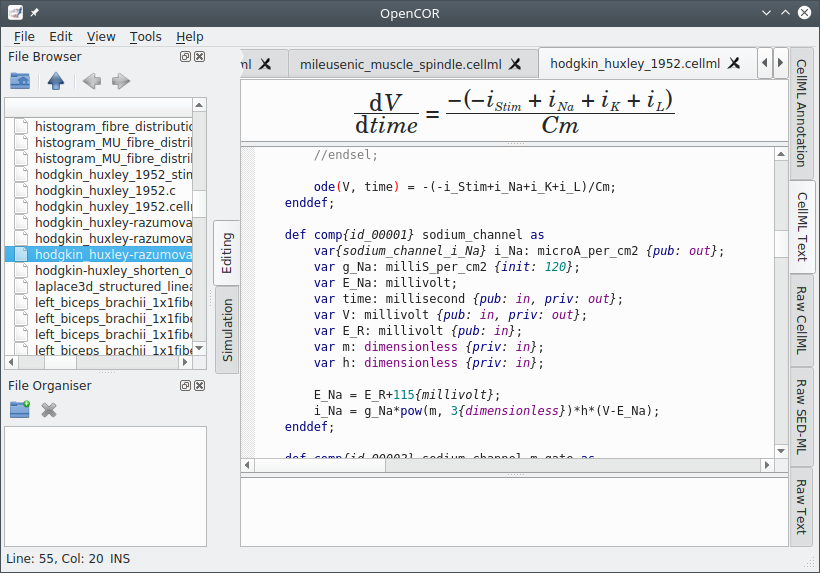
\includegraphics[width=\textwidth]{images/implementation/opencor1.png}
    \caption{CellML editor with the ODE for the membrane voltage \say{V} in the Hodgkin-Huxley cellular model, which corresponds to \cref{eq:subcellular_model_helper4} inserted into \cref{eq:subcellular_model_helper3}.}%
    \label{fig:opencor1}%
  \end{subfigure}
  \quad
  \begin{subfigure}[t]{0.45\textwidth}%
    \centering%
    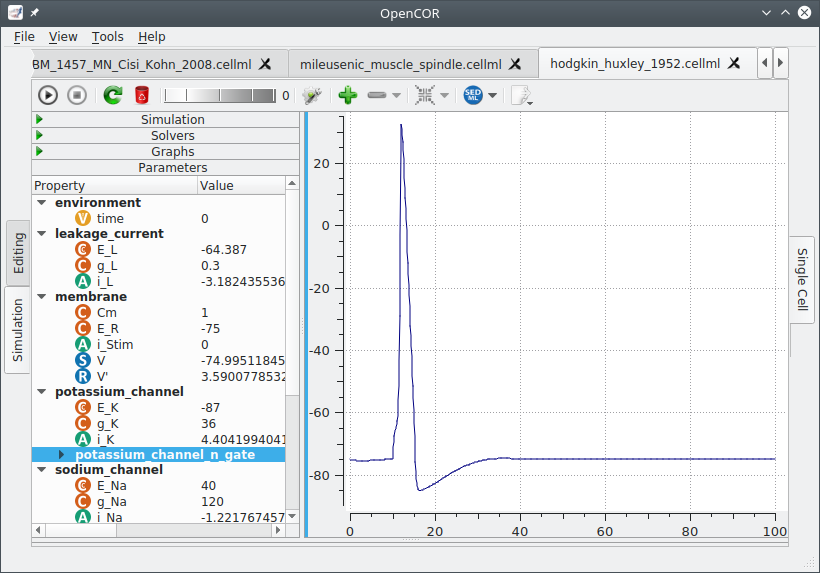
\includegraphics[width=\textwidth]{images/implementation/opencor2.png}
    \caption{Visualization of a simulated action potential $V_m$ over time.}%
    \label{fig:opencor2}%
  \end{subfigure}
  \caption{The CellML modeling environment OpenCOR.}%
  \label{fig:opencor}%
\end{figure}%

\emph{OpenCOR} \cite{OpenCOR2015} provides a modeling environment in a graphical user interface, where models can be edited. 
\Cref{fig:opencor1} shows the interface with the editor on the right. Mathematical equations are described in a declarative language and can be rendered to mathematical notation, as seen in the upper part in \cref{fig:opencor1}. OpenCOR automatically transfers the equations to the XML-based MathML syntax and integrates them in the XML-based CellML description.
OpenCOR can also be used to solve the system of DAEs using implicit solvers such as backward differentiation formulas. The solver parameters can be adjusted and the solver can be started from the graphical user interface. \Cref{fig:opencor2} shows the interface that lists all variables with their current values on the left and a visualization of the result, in this case an action potential, on the right.

OpenCOR also provides command line functionality to convert CellML files into C code. This generated C code can evaluate all model equations but not solve the DAE system. Because OpenCOR is robust and well established in the bioengineering modeling community, we decide to use it in OpenDiHu. The installation procedure of OpenDiHu downloads and installs OpenCOR automatically.

During execution of a simulation, our framework parses the C code of CellML models, compiles a shared library and executes the functions, all at runtime. Thus, the CellML model can be directly given as a C file. Otherwise, if the model file is in XML format, it is assumed to be a CellML description and automatically converted to the required C code using the OpenCOR command line interface.

If a CellML model is manually simulated in the OpenCOR graphical user interface with time-varying input signals, these signals have to be hard-coded in the model, e.g., as a piecewise defined function. This is acceptable for getting insight into the models, but counteracts the idea of modular models that can be shared and recombined. 
As a remedy, we design our framework in a way that simulations of CellML models with configurable time-varying input signals are possible without the need to change the CellML description.

CellML models are limited to single-cell systems of DAEs and are not designed for PDEs that, e.g., involve multiple instances of a DAE system on a given geometry. Thus, the monodomain equation cannot be solved with OpenCOR and a multi-scale software framework is needed for this task. Two such frameworks with CellML support, which were described in the introduction in \cref{sec:intro_related_software}, are Chaste and OpenCMISS Iron. In the following, we relate and compare the approaches of CellML integration in OpenDiHu and these existing frameworks.

\begin{table}
  \centering%
  \begin{tabular}{|c|l|l|l|l|l|}
    \hline
    Symbol        & \multicolumn{3}{l|}{Name}            & Computed          & Initial values\\
    \cline{2-4}
                  & OpenCOR    & OpenCMISS & OpenDiHu   & by model?          & can be set?\\
    \hline
    $\bfy$        & \code{state}     & \code{STATES}    & \code{state}     & by timestepping   & yes \\[2mm]
    $\partial\bfy/\partial t$ & \code{rate}      & \code{RATES}     & \code{rate}      & yes               & no  \\[2mm]
    $\hat{\bfc}$  & \code{constant}  & \code{CONSTANTS} & \code{constant}  & no                &in CellML  \\[2mm]
    $\bfh$        & \code{algebraic}  & \code{WANTED}    & \code{algebraic} & yes               & no  \\[2mm]
    $\hat{\bfp}$  & -  & \code{KNOWN}     & \code{parameter} & no                & yes \\
    \hline
  \end{tabular}
  \caption{The different CellML quantities and their properties and names in various tools.}%
  \label{tab:cellml_names}%
\end{table}

The variables in the generic DAE in \cref{eq:cellml_generic_dae} have different names in the different software packages. \Cref{tab:cellml_names} compares the symbols and their names in OpenCOR, OpenCMISS in OpenDiHu and summarized how their values are determined. 

All three software packages have the concept of \code{state} and \code{rate} vectors, where the states $\bfy$ are the input and the rates $\partial\bfy/\partial t$ are the output of the CellML formulas. Similarly, the constants $\hat{\bfc}$ are always a set of predefined values that are fixed during the computations.

The algebraic formulas lead to the values in $\bfh$, independently of the timestepping scheme. These algebraic values can be considered as the resulting quantities of interest of the model and are typically written to output files or transferred to coupled solvers.

Moreover, OpenCMISS and OpenDiHu define parameters $\hat{\bfp}$, which influence the behavior of the model. Their values can be changed by a coupled solver or prescribed from the settings. 
In OpenDiHu, any constant or algebraic variable in a CellML model can be converted into a parameter. All occurrences of the constant or algebraic variable in the CellML description get replaced by the parameter variable. For former algebraic variables, this replacement step overrides the equations that would have defined the algebraic value. Exemplary use cases are to set the external stimulation current $I_\text{ext}$ in \cref{eq:subcellular_model_helper3} or to set the fiber stretch in a strain-dependent subcellular model.

OpenCMISS uses a similar concept, where some algebraics in the CellML description can be declared as \code{WANTED} to be read by the framework. Some of the constants can be declared as \code{KNOWN} such that OpenCMISS sets their values from other computations within OpenCMISS. (Assigning new values to algebraics as in OpenDiHu is not possible.) Because the terms \code{WANTED} and \code{KNOWN} can be ambiguous if either seen from within the CellML model or from the framework, we decide to use the terms \code{algebraics} and \code{parameters} instead.

The last two columns of \cref{tab:cellml_names} summarize the purpose of the different quantities. The CellML description defines formulas for the states, rates and algebraics. Rates and algebraics are directly calculated by the code that is generated from the CellML model, the vector of states is then computed from the vector of rates by the timestepping scheme. The initial values of the states are either explicitly specified in the OpenDiHu settings, e.g., to allow different values for different instances of a model. Or, if this specification is omitted,  the initial values are set according to the specification in the CellML file. The parameter values always have to be specified in the Python settings. By definition, the constants cannot be set from OpenDiHu, but are given in the CellML model. If the value of a constant should be specified from the settings, the variable should instead be configured to be a parameter.


From a computational point of view, a CellML model computes the following function in terms of the introduced variable names:
\begin{equation}
  \left(
    \begin{array}{cc}
      \texttt{rates} \\ \texttt{algebraics} 
    \end{array}
  \right) = \texttt{cellml}\left(\texttt{states}, \texttt{constants}\right).
  \label{eq:cellml_generic}
\end{equation}

In the fiber based electrophysiology model, CellML is needed to formulate the reaction term in the monodomain equation \cref{eq:monodomain}, which is repeated here:
\begin{align}\label{eq:monodomain_2}
  \p{V_m}{t}  = \dfrac{\sigma_\text{eff}}{A_m\,C_m} \p{V_m}{x}{2} - \dfrac{1}{C_m} I_\text{ion}(V_m,\bfy).
\end{align}
The \code{states} vector in \cref{eq:cellml_generic} includes both $V_m$ and $\bfy$ in \cref{eq:monodomain_2}. In consequence, the computed \code{rates} contain $\partial V_m/\partial t$ and $\partial\bfy/\partial t$. The right-hand side of \cref{eq:cellml_generic}, i.e., the \code{cellml} function calculates the term $(-1/C_m \cdot I_\text{ion})$, which is the reaction part of the monodomain equation in \cref{eq:monodomain_2}. Thus, the CellML computation can be directly used in the operator splitting approach in \cref{sec:discretization_monodomain}.

For the solution of CellML models, OpenCMISS implements the explicit forward Euler scheme or allows to use the backward differentiation formula (BDF) schemes with adaptive order of convergence of SUNDIALS. Recently, an implementation of the second order explicit Heun scheme was added by Aaron Krämer. Accuracy and runtimes were investigated for Euler, Heun and BDF solvers for the subcellular model within the monodomain equation. Because of the operator splitting scheme, only very small timespans have to be solved by those solvers, which does not redeem the overhead of advanced schemes such as the BDF solver, ultimately yielding the best performance for the Heun solver. Based on these investigations, we choose to implement the forward Euler and Heun schemes for the solution of CellML models in OpenDiHu.

% comparison to Chaste
The following differences exist between the approaches to support CellML models in Chaste, OpenCMISS Iron and OpenDiHu:
Chaste tries to automatically determine the CellML variable names of standard quantities such as the membrane voltage and the stimulation current. This requires potentially less user intervention when CellML models are exchanged.
In OpenDiHu, the step of identifying the CellML variables to be connected to the coupled solvers is done manually to give the user complete control over the setup. It can be achieved in a clear way with the Python settings script. Another difference in OpenDiHu is that all computational code is guaranteed to invoke vector instructions, i.e., following the single-instruction multiple data (SIMD) paradigm. Chaste only relies on the optimization behavior of the Intel compiler, which is not guaranteed to be optimal, e.g., for non-Intel hardware.

% comparison to Iron
The computational core Iron from the OpenCMISS package employs the CellML API and also requires manual connections of CellML variables to the solver code. These variable mappings have to be hard-coded in the main Fortran program (if the Python wrappers are not used) and are compiled into the program. Thus, a CellML model is a fixed part of a compiled simulation program. In contrast, OpenDiHu allows to configure the CellML model at runtime.
Another difference in the implementation is that Iron uses a non-optimal memory layout for the state vector, which prohibits vectorization and slows down the solution compared to OpenDiHu.

\subsection{Mapping of CellML Variables to Slots and Parameters}

Preparing the OpenDiHu solver for use with a CellML model consists of the two steps of adjusting the C++ template parameters and setting up the variable mappings in the Python settings. The two C++ template parameters have to be set to the sizes of the state vector $\bfy$ and the algebraics vector $\bfh$. The code snipped in \cref{fig:example_shorten_cellml} belongs to the example program in \code{examples/electrophysiology/cellml/shorten}, which solves a single-cell CellML model:
\begin{figure}[H]
\centering
\begin{framed}
\begin{lstlisting}[basicstyle=\small\ttfamily,commentstyle=\color{gray},numbers=left]
  TimeSteppingScheme::ExplicitEuler<
    CellmlAdapter<56,71>
  >
\end{lstlisting}
\end{framed}
\caption{C++ code snipped that solves a CellML model with an explicit Euler scheme. The two template parameters 56 and 71 correspond to the number of states and algebraics, respectively.}%
\label{fig:example_shorten_cellml}%
\end{figure}
In this case, the model contains 56 states and 71 algebraics. The reason that these numbers have to be fixed at compile-time is that this allows the data structures in the implementation to have a fixed layout and be allocated on the stack instead of the heap, which improves the performance.

If the given numbers are not matching the variables in the CellML file, appropriate warnings or errors are generated, containing the correct C++ code to be copied to the C++ file. If the numbers are too high, the solver still works correctly, however, some memory and computation time is wasted for the excess variables.

The other step is configuring the connections between the CellML computation and input data or coupled solvers. This involves defining a \code{mappings} parameter. \Cref{fig:example_mapping} shows such a definition for the multidomain example with fat layer and a contraction model, which was presented in \cref{sec:exemplary_usage_2}.

\begin{figure}
\centering
\begin{framed}
%\begin{Verbatim}[fontsize=\small]
\begin{lstlisting}[basicstyle=\small\ttfamily,commentstyle=\color{gray},numbers=left,language=python]
  mappings = {
    # function in OpenDiHu      name in CellML model    # comment
    
    ("parameter", 0):           "wal_environment/I_HH", # I_stim (constant)   $\label{alg:5.3}$
    ("parameter", 1):           "razumova/L_S",         # $\textcolor{gray}{\lambda}$ (constant)      $\label{alg:5.4}$
    
    ("connectorSlot", "vm"):    "wal_environment/vS",   # $\textcolor{gray}{V_m}$ (state)            $\label{alg:5.7}$
    ("connectorSlot", "stress"):"razumova/stress",      # $\textcolor{gray}{\gamma}$ (algebraic) $\label{alg:5.8}$
    ("connectorSlot", "lambda"):"razumova/L_S",         # $\textcolor{gray}{\lambda}$ (constant)        $\label{alg:5.9}$
  }
  
  parameters_initial_values = [0.0, 1.0]                # I_stim=0, $\textcolor{gray}{\lambda}$=1                    $\label{alg:5.12}$
\end{lstlisting}
%\end{Verbatim}
\end{framed}
\caption{Specification of parameters and connector slots in a CellML model. The listed settings define two CellML variables to be parameters and specify three connector slots to transfer values between coupled solvers.}%
\label{fig:example_mapping}%
\end{figure}

The \code{mappings} define which CellML constants or algebraics are treated as parameters. Lines \ref{alg:5.3} and \ref{alg:5.4} make the stimulation current and fiber stretch constants accessible from outside the CellML model by making them parameters. The variables are identified by their names and the model components they are defined in in the CellML model. In this example, the first parameter is the stimulation current \code{I_HH} within the \code{wal_environment} model component and the second parameter is the fiber stretch or half-sarcomere length \code{L_S} in the \code{razumova} component.
The initial values for these parameters are given in line \ref{alg:5.12}, which sets the stimulation current to zero and the fiber stretch to one.

The second information in the \code{mappings} parameter is which variables from the CellML model are exposed to coupled solvers in OpenDiHu. This happens by defining connector slots that can be connected between the solvers as shown in \cref{fig:example_multidomain_solver_structure}.
Three slots are defined in lines \ref{alg:5.7} to \ref{alg:5.9} with slot names \code{`vm`}, \code{`stress`} and \code{`lambda`}. The corresponding CellML variables are again specified by their model component name and their own name. 

CellML variables of all three different types are connected in the example. The membrane voltage $V_m$ in slot \code{`vm`} is part of the state vector $\bfy$. In this example, it is used in a bidirectional coupling with the diffusion solver. The second slot, \code{`stress`}, connects to the activation parameter $\gamma$, which is part of the algebraic vector $\bfh$. It is an output of the model. The slot \code{`lambda`} refers to a constant in the CellML description, which has been transformed to a parameter in line \ref{alg:5.4}. It is used as an  input and the received values at these slots are moved to the corresponding locations in the CellML formulation.


\subsection{Consistent Physical Units in CellML Models and the Multi-Scale Framework}

The variables in a CellML model describe physical quantities. CellML handles their physical units and computes the appropriate conversions when combining model components within a CellML description.
For the integration of a CellML model in external solvers such as OpenDiHu, we have to take care that the units are consistent.

\sisetup{retain-unity-mantissa = false}
The subcellular models that we use are formulated with the following units for length, time, electric current and capacitance:%
\begin{align*}
   \SI{1}{\centi\meter} &= \SI{1e-2}{\meter}, &
   \SI{1}{\milli\second} &= \SI{1e-3}{\second}, &
   \SI{1}{\micro\ampere} &= \SI{1e-6}{\ampere}, &
   \SI{1}{\micro\farad} = \SI{1e-6}{\farad}.
\end{align*}
These basic units also fix derived units such as \SI{1}{\kilo\hertz} for frequencies and \SI{1}{\milli\volt} for voltages. For example, the membrane capacitance $C_m$ has to be specified in units \SI{1}{\micro\farad\per\square\centi\meter} and the stimulation current $I_\text{stim}$ in the units \SI{1}{\micro\ampere\per\square\centi\meter}.

With this system of units, values are in a similar scale when computing subcellular models. However, these units are less suitable for organ-scale computations, as the derived mass and density units are \SI{1e-14}{\kilogram} and \SI{1e-8}{\kilogram\per\meter\cubed} and the derived force and stress units are \SI{1e-10}{\newton} and \SI{1e-6}{\pascal}. For the dynamic solid mechanics model, where these quantities play a role, we use the following different system of units:
\begin{align*}
   \SI{1}{\centi\meter} &= \SI{1e-2}{\meter}, &
   \SI{1}{\milli\second} &= \SI{1e-3}{\second}, &
   \SI{1}{\newton}.
\end{align*}
The length and time scales are identical to the subcellular model and allow for consistent coupling. The coupling of active stresses from the subcellular model to the solid mechanics model uses the unit-less activation parameter $\gamma \in [0,1]$, which is transferred to stress units by multiplication with a maximum active stress value in the solid mechanics model.

Derived units in the solid mechanics system of units are \SI{1e2}{\kilogram\per\meter\cubed} for the density, \SI{1e4}{\meter\per\square\second} for the acceleration and $\SI{1}{\newton\per\square\centi\meter} = \SI{10}{\kilo\pascal}$ for the stress. The values of material parameters and boundary conditions have to be given with respect to these units.
The units allow for smaller values in the solid mechanics computation than in the unit system of the subcellular model. Moreover, it is  convenient to specify forces directly in terms of \SI{1}{\newton}.

% # Fixed units in cellMl models:
% # These define the unit system.
% # 1 cm = 1e-2 m
% # 1 ms = 1e-3 s
% # 1 uA = 1e-6 A
% # 1 uF = 1e-6 F
% # 
% # derived units:
% #   (F=s^4*A^2*m^-2*kg^-1) => 1 ms^4*uA^2*cm^-2*x*kg^-1 = (1e-3)^4 s^4 * (1e-6)^2 A^2 * (1e-2)^-2 m^-2 * (x)^-1 kg^-1 = 1e-12 * 1e-12 * 1e4 F = 1e-20 * x^-1 F := 1e-6 F => x = 1e-14
% # 1e-14 kg = 10e-15 kg = 10e-12 g = 10 pg
% 
% # (N=kg*m*s^-2) => 1 10pg*cm*ms^2 = 1e-14 kg * 1e-2 m * (1e-3)^-2 s^-2 = 1e-14 * 1e-2 * 1e6 N = 1e-10 N = 10 nN
% # (S=kg^-1*m^-2*s^3*A^2, Siemens not Sievert!) => (1e-14*kg)^-1*cm^-2*ms^3*uA^2 = (1e-14)^-1 kg^-1 * (1e-2)^-2 m^-2 * (1e-3)^3 s^3 * (1e-6)^2 A^2 = 1e14 * 1e4 * 1e-9 * 1e-12 S = 1e-3 S = 1 mS
% # (V=kg*m^2*s^-3*A^-1) => 1 10pg*cm^2*ms^-3*uA^-1 = (1e-14) kg * (1e-2)^2 m^2 * (1e-3)^-3 s^-3 * (1e-6)^-1 A^-1 = 1e-14 * 1e-4 * 1e6 * 1e6 V = 1e-6 V = 1mV
% # (Hz=s^-1) => 1 ms^-1 = (1e-3)^-1 s^-1 = 1e3 Hz
% # (kg/m^3) => 1 10 pg/cm^3 = 1e-14 kg / (1e-2 m)^3 = 1e-14 * 1e6 kg/m^3 = 1e-8 kg/m^3
% # (Pa=kg/(m*s^2)) => 1e-14 kg / (1e-2 m * 1e-3^2 s^2) = 1e-14 / (1e-8) Pa = 1e-6 Pa
% 
% # Hodgkin-Huxley
% # t: ms
% # STATES[0], Vm: mV
% # CONSTANTS[1], Cm: uF*cm^-2
% # CONSTANTS[2], I_Stim: uA*cm^-2
% # -> all units are consistent
% 
% # Shorten
% # t: ms
% # CONSTANTS[0], Cm: uF*cm^-2
% # STATES[0], Vm: mV
% # ALGEBRAIC[32], I_Stim: uA*cm^-2
% # -> all units are consistent
% 
% # Fixed units in mechanics system
% # 1 cm = 1e-2 m
% # 1 ms = 1e-3 s
% # 1 N
% # 1 N/cm^2 = (kg*m*s^-2) / (1e-2 m)^2 = 1e4 kg*m^-1*s^-2 = 10 kPa
% # (kg = N*s^2*m^-1) => N*ms^2*cm^-1 = N*(1e-3 s)^2 * (1e-2 m)^-1 = 1e-4 N*s^2*m^-1 = 1e-4 kg
% # (kg/m^3) => 1 * 1e-4 kg * (1e-2 m)^-3 = 1e2 kg/m^3
% # (m/s^2) => 1 cm/ms^2 = 1e-2 m * (1e-3 s)^-2 = 1e4 m*s^-2

\subsection{Specification of Stimulation Times Using Callback Functions}\label{sec:stimulation_times_callbacks}

A muscle fiber is activated by impulse trains that are generated from a motor neuron and stimulate the fiber at its neuromuscular junction. At the synaptic terminal, neurotransmitters are released and open certain ion channels, which results in depolarization of the muscle fiber membrane.
This process can either be modeled by adding an external stimulation current $I_\text{stim}$ through the dedicated ion channels or by directly prescribing the transmembrane voltage $V_m$ to reflect the resulting depolarized state. The first approach is more accurate as it also describes the depolarization process at the stimulated parts of the fiber. The electric \say{far field} away from the stimulation point, however, is the same for both approaches.

In OpenDiHu, it is possible to configure either approach. Setting the stimulation current is more involved as the actual value of  $I_\text{stim}$ has to be chosen depending on the mesh width. Furthermore, multiple adjacent nodes have to be stimulated such that the electric current that is added to the system balances with the amount that is carried away by the diffusion term. The nonlinear subcellular model fails to compute a valid solution, if too much current is present. With too little current, the membrane potential stays below the activation threshold and no action potential is triggered. 

Prescribing the transmembrane voltage to a value above the depolarization threshold at multiple adjacent nodes leads to equivalent action potentials independent of the mesh width. However, a suitable value for the prescribed voltage also has to be chosen in accordance with the employed subcellular model.

The stimulation current $I_\text{stim}$ is a CellML parameter and the transmembrane voltage $V_m$ corresponds to a state in the CellML model. The values of both parameters and states can be adjusted during the simulation. This feature is implemented by means of callback functions in the Python settings. A callback is a user defined function that gets called in regular intervals during the simulation, receives various information about the current state of the simulation and can alter some values such as the states vector $\bfy(t)$ or the parameters vector $\hat{\bfp}(t)$.

\begin{figure}
\centering
\begin{framed}
%\begin{Verbatim}[fontsize=\small]
\begin{lstlisting}[basicstyle=\footnotesize\ttfamily,commentstyle=\color{gray},numbers=left,language=python]

  # callback function that can set parameters, i.e. stimulation current
  def $\textcolor{Maroon}{\text{\ttfamily set\_specific\_parameters}}$(n_nodes_global, time_step_no, current_time, $\label{alg:6.3}$
                              parameters, fiber_no):    
    
    # determine if fiber gets stimulated at the current time
    if fiber_gets_stimulated(fiber_no, current_time):    $\label{alg:6.6}$
      stimulation_current = 40.
    else:
      stimulation_current = 0.

    innervation_node_global = int(n_nodes_global / 2)    $\label{alg:6.11}$
    parameters[(innervation_node_global),0,0] = stimulation_current    $\label{alg:6.12}$

  # callback function that can set states, e.g., prescribe $\textcolor{gray}{V_m}$ for stimulation
  def $\textcolor{Maroon}{\text{\ttfamily set\_specific\_states}}$(n_nodes_global, time_step_no, current_time,       $\label{alg:6.15}$
                          states, fiber_no):            

    # determine if fiber gets stimulated at the current time
    if fiber_gets_stimulated(fiber_no, current_time):    $\label{alg:6.18}$
      innervation_node_global = int(n_nodes_global / 2)    $\label{alg:6.19}$
      states[(innervation_node_global),0,0] = 40.0      $\label{alg:6.20}$

  config = {        $\label{alg:6.22}$
    (...)          
    
    # callback to adjust parameters
    "setSpecificParametersFunction":         $\textcolor{Maroon}{\text{\ttfamily set\_specific\_parameters}}$,    $\label{alg:6.28}$
    "setSpecificParametersCallInterval":     1e3,
    "setSpecificStatesFrequencyJitter":      0,                          
                    
    # callback to alter values of states
    "setSpecificStatesFunction":             $\textcolor{Maroon}{\text{\ttfamily set\_specific\_states}}$,      $\label{alg:6.33}$
    "setSpecificStatesCallInterval":         2*int(1/stimulation_frequency/dt_0D),     $\label{alg:6.34}$
    
    "setSpecificStatesCallFrequency":        stimulation_frequency,    $\label{alg:6.36}$
    "setSpecificStatesCallEnableBegin":      0,                        $\label{alg:6.37}$
    "setSpecificStatesRepeatAfterFirstCall": 0.01,                     $\label{alg:6.38}$
    "setSpecificStatesFrequencyJitter":      [0.1,-0.2,0.0],           $\label{alg:6.39}$
                         
    # callback to postprocess the result
    "handleResultFunction":                  $\textcolor{Maroon}{\text{\ttfamily handle\_result}}$,    $\label{alg:6.41}$
    "handleResultCallInterval":              1e4,         
     
    "additionalArgument":                    fiber_no,        $\label{alg:6.43}$
  }

\end{lstlisting}
%\end{Verbatim}
\end{framed}
\caption{Settings that define neural spike trains activating muscle fibers. The definition of the two callback functions \code{set_specific_parameters} and \code{set_specific_states} is demonstrated.}%
\label{fig:example_callback_functions}%
\end{figure}

\Cref{fig:example_callback_functions} defines two such callback functions used in the fiber based electrophysiology model to add electric stimulation to the monodomain model. Either suffices to implement the stimulation. The function \code{set_specific_parameters} in line \ref{alg:6.3} and the function \code{set_specific_states} in line \ref{alg:6.15} both receive similar information from the simulation as their function arguments: the total number \code{n_nodes_global} of nodes in the current fiber, the current integer timestep number \code{time_step_no}, the corresponding floating-point number \code{current_time} of the current simulation time, and the number \code{fiber_no} that identifies the current fiber.

The variables \code{parameters} and \code{states} are the output of the callback functions that alter the parameter and state values, respectively. Both callbacks determine, whether the current fiber should be stimulated at the current time, in lines \ref{alg:6.6} and \ref{alg:6.18}.
If yes, the parameter or state at the center point of the fiber, computed in lines \ref{alg:6.11} and \ref{alg:6.19}, gets changed accordingly. In the real scenario, three adjacent points get stimulated instead of a single point.

Because the conversion of transferred data between the Python code and the C++ code costs some runtime, the number of transferred values is reduced to a minimum. Only the parameters and states that should be changed are indicated in the \code{parameters} and \code{states} variables in lines \ref{alg:6.12} and \ref{alg:6.20}. These variables are Python dictionaries, i.e., key-value pairs. The key is a tuple of three items: First, the global coordinates $(x,y,z)$ of the node where the parameter or state change is applied. In case of a 1D fiber mesh, this is only a single coordinate. Second, the dof index on this node. This is different from zero only for Hermite ansatz functions, which have multiple dofs per node. And third, the index of the parameter or state that should be set. Parameter 0 corresponds to the stimulation current as defined in line \ref{alg:5.3} of \cref{fig:example_mapping}, and state 0 corresponds to the transmembrane voltage $V_m$. The new value to set is the value of the key-value pair.

The comparison of the two callbacks functions shows one difference: In the callback for the parameters, the stimulation current is set to zero when there is no stimulation. In the callback for the states, nothing is done during this time. The reason for this is that the state values will be continuously updated from the rates by the timestepping scheme, whereas the parameters keep their values until they are changed from the callback. This has consequences on the times at which the callback functions have to be called from the simulation, which are described in the following.

Invoking the Python interpreter on a callback requires some time. Calling the callback after every small timestep of the simulation is, thus, not performant. We model the stimulation of a fiber by a piecewise constant function with two possible values for on and off.
In the approach that sets the stimulation current, the callback \code{set_specific_parameters} has to be called at the onset and at the end of every stimulation spike. If the approach with the prescribed membrane voltage is used, the callback \code{set_specific_states} has to be called after every stimulation onset in every subsequent timestep until the stimulation is over.

The requirements for both approaches can be satisfied by defining a small constant interval of timesteps after which the callback functions are invoked. This call interval can be specified in the \code{config} dictionary of the Python file in \cref{fig:example_callback_functions} , which is shown in excerpts from line \ref{alg:6.22} onwards. The \code{config} variable references the callback functions in lines \ref{alg:6.28} and \ref{alg:6.33} and the parameters for the call interval in the next lines. Note that this configuration is only shown for demonstration, a real configuration should either specify the states callback or the parameters callback function, not both.

Line \ref{alg:6.34} in \cref{fig:example_callback_functions} shows how the call interval can be computed to correspond to a given stimulation frequency \code{stimulation_frequency}, given the timestep width \code{dt_0D}. The prefactor of two occurs because the callback would be called twice per timestep in the Strang splitting scheme.

Real impulse trains from the motor neuron pool typically follow a base frequency with some added jitter that offsets the exact firing times from the base frequency by a small random time. Furthermore, studies are often designed to start with a completely inactive muscle and switch on certain MUs after specified times. To efficiently account for these two demands, we add another way to specify the times when the \code{set_specific_states} callback gets invoked. In this second way of specification, the \code{setSpecificStatesCallInterval} parameter is disabled by setting it to zero. Then, the three options \code{CallFrequency}, \code{CallEnableBegin}, \code{RepeatAfterFirstCall} and \code{Frequency}\code{Jitter} (prefixed by \code{set}\code{Specific}\code{States}) given in lines \ref{alg:6.36} to \ref{alg:6.39} are significant. 

\begin{figure}%
  \centering%
  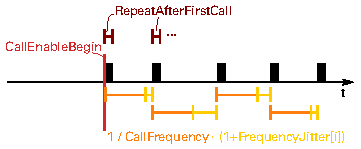
\includegraphics[width=0.8\textwidth]{images/implementation/stimulation_times.pdf}%
  \caption{Parametrization of stimulation times in electrophysiology simulations. The neuronal impulse train is given by the black spikes. The parameters \code{CallEnableBegin}, \code{RepeatAfterFirstCall}, \code{CallFrequency} and \code{FrequencyJitter} (in the settings all prefixed by \code{setSpecificStates}) specify the shape of the spike train.}%
  \label{fig:stimulation_times}%
\end{figure}%

Their meaning is illustrated in \cref{fig:stimulation_times}. \code{CallEnableBegin} specifies the time when the callback should be called for the first time. Then, it is called with a frequency that is additively composed of the base frequency given by \code{CallFrequency} and one entry of the parameter \code{FrequencyJitter}. This parameter is a ring buffer of relative factors by which the regular time span between subsequent firing events is prolonged. For example, if \code{FrequencyJitter} contains the list \code{[0.1,-0.2,0.0]}, the time span $T_{01}$ between the first two firing events is \SI{10}{\percent} longer than according to the base frequency $f$, the next timespan $T_{12}$ is \SI{20}{\percent} shorter and the next time span $T_{23}$ exactly equals the inverse base frequency, $T_{23} = 1/f$. Subsequently, the scheme repeats. Typically, this parameter is set to a randomly generated list with a large number of entries.
After each onset of a stimulation, the \code{setSpecificStatesCallInterval} function is called repeatedly in every subsequent timestep for a time span given by \code{RepeatAfterFirstCall}. 

In the fiber based electrophysiology example, every fiber has its own instance of the Python settings, and it is possible to specify different parameter values for different fibers or motor units, e.g., to set a different beginning time of the stimulations. The fibers can be distinguished by the last parameter of the callbacks, which receives the custom value that is defined by the \code{`additionalArgument`} parameter in line \ref{alg:6.43}. In the given example, the current fiber number is used here, but any other Python variable is possible.

\Cref{fig:firing_times_ramp} shows a scenario, where different parameters are set for different MUs. The figure shows the firing times of fibers grouped to 20 MUs, which are activated in a ramp in the first $t=\SI{19}{\second}$. The base frequency decreases from \SI{23.92}{\hertz} to \SI{7.66}{\hertz} for MUs 1 to 20, which reproduces a scenario in literature \cite{Klotz2020}. The frequency jitter parameter is a list of 100 randomly chosen values between \SI{-10}{\percent} and \SI[retain-explicit-plus]{+10}{\percent}. The \code{CallEnableBegin} parameter enables the stimulation of the next MU every second.

\begin{figure}%
  \centering%
  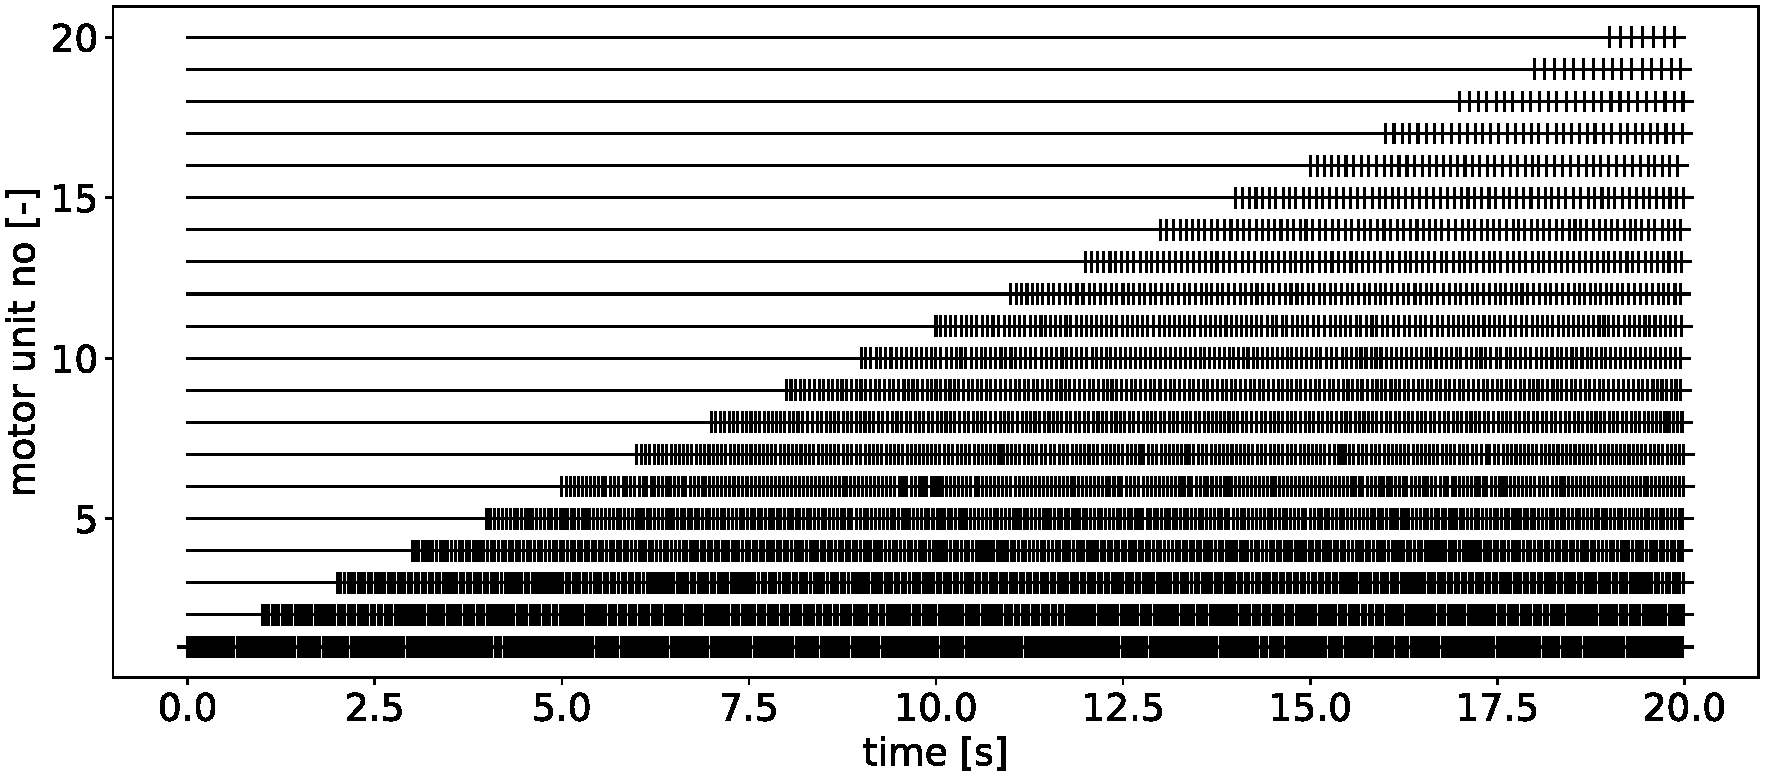
\includegraphics[width=\textwidth]{images/implementation/firing_times_ramp1.pdf}%
  \caption{Firing times for a scenario with 20 motor units with ramp-like activation and different stimulation frequencies.}%
  \label{fig:firing_times_ramp}%
\end{figure}%

Similar to the two presented callbacks, which set parameters and states, a third callback \code{handle_result} can be defined as given in line \ref{alg:6.41} of \cref{fig:example_callback_functions}. This callback function gets called in a fixed interval specified by \code{`handleResultCallInterval`}. It receives the complete vectors of states $\bfy$ and intermediates $\bfh$ and can be used to perform custom post-processing or to output custom data files from the Python script.

In summary, variables of CellML models can be coupled to other solvers. Their parameters and values can be adjusted from the settings file. Callback functions are used to alter values during the simulation. This flexibility comes at the runtime cost of invoking the Python interpreter, therefore the times when to call the callback functions have to be specified appropriately. Special methods exist to model steady stimulation with frequency jitter, which occurs in typical neural stimulation of muscle fibers.

% --------------------------------------------
\section{Output File Formats}\label{sec:output_file_formats}

After the simulation program completes, the computed results can be visualized using external tools.
As mentioned in the previous sections, output writers are used to generate output files in various formats. The formats of the output writers and additional options are configured in the Python settings under the parameter \code{OutputWriter}. The following formats are supported:\code{`ParaView`}, \code{`ExFile`}, \code{`PythonFile`}, \code{`PythonCallback`} and\break\code{`MegaMol`}.
The corresponding output can be visualized and post-processed using different tools, which will be presented in the following. We use simulation results of a fiber-based electrophysiology scenario with 49 1D fibers and a 3D muscle mesh to showcase the different output data formats.

\subsection{Output of VTK Files for the Use with ParaView}
The canonical way to visualize simulation results computed by OpenDiHu is to use the software ParaView \cite{paraview}. 
The required output file formats are defined by the Visualization Toolkit (VTK) specification \cite{vtk}. Depending on the mesh type in OpenDiHu, different file types are generated:
\emph{RectilinearGrid} files (with file ending \code{.vtr}) for the output of \say{regular fixed} meshes that represent a cartesian grid,
\emph{StructuredGrid} files (\code{.vts}) for the output of \say{structured deformable} meshes, i.e., structured meshes that can deform over time, 
\emph{UnstructuredGrid} files (\code{.vtu}) for the output of unstructured meshes, and
\emph{PolyData} files (\code{.vtp}) containing connected points are used to represent multiple muscle fibers in a single file.
ParaView can be used to load and visualize all of these file types.

All of these files are XML based and their payload data can be configured to be either written in ASCII representation or in Base64 encoding. Base64 encoding also translates the raw data into ASCII characters. The data stream is split into pieces of 6 bits, which are each represented by an 8-bit-ASCII character. Thus, the required memory is $4/3$ of the raw data. Compared to a full ASCII representation containing the digits of all numerical values, this leads to a significant reduction of file sizes.

The VTK file format specifies parallel file output, where each process writes its local data to a separate file and one additional master file references the pieces in all files. This parallel file output scheme is implemented in OpenDiHu. However, it can lead to an impractically large number of small output files for high degrees of parallelism. 

Therefore, we additionally implement a second approach, where non-parallel VTK files, which contain the whole dataset, are written. The same type of output files is generated during serial and parallel execution of the program. 
Writing the data to such a file is done using the parallel output capabilities of MPI. The respective MPI functions allow to collectively write data to the same file from different processes at different locations in the file. For parallel execution, every process only writes its own local data and no communication of the payload data to a master process is necessary. 

Because the byte boundaries in a Base64 encoded data stream coincide with multiples of 8 bits only every three bytes, the processes that write neighboring parts in the output file have to coordinate the bit offsets of their data streams. For this, a small amount of data has to be communicated between these processes. However, the cost of this communication is negligible.

With this improved output scheme, one file is generated per mesh and output timestep of the simulation. The frequency of output timesteps can be configured in the Python settings.
It is also possible and useful to combine all 1D fiber meshes into a single output file per timestep to reduce the number of output files.

Different meshes can be written with different frequency. For example, for a simulation of fiber based electrophysiology with EMG signals, it is reasonable to output the comprehensive dataset of all fibers less frequently than the smaller dataset of EMG signals on the 2D skin surface. To associate the output files with the correct times, a timestamp of the current simulation time is added to every file. Furthermore, partitioning information is added, i.e., which part of the mesh is computed by which process.

To synchronize output files of different meshes with different output frequencies in the visualization tool, additional \emph{series files} (with file ending \code{.series}) are automatically created for every mesh. Such a file references all available output files of a mesh with their simulation times in JSON format. These files can be opened in ParaView to get a time-series of the simulation result.

Using the series files is also convenient, if the simulation is run in a directory, where old simulation results from previous runs exist. Because the series files are updated every timestep and only reference the newly created files, opening these files in ParaView only visualizes newly created simulation output, in contrast to opening a whole directory, which would potentially also load old results.

\subsection{Visualization With ParaView}
ParaView allows various manipulations and types of visualization of the loaded data. \Cref{fig:paraview_output} shows the ParaView window with simulation data of a fiber-based electrophysiology scenario. The loaded data are organized in a tree of datasets with applied filters, which can be seen in the \say{Pipeline Browser} in the top left. The center view shows a visualization of the muscle fibers and the 3D mesh at simulation time $t=\SI{89.6}{\milli\second}$. An animation of the transient data can be shown by using the playback controls in the top bar.

\begin{figure}%
  \centering%
  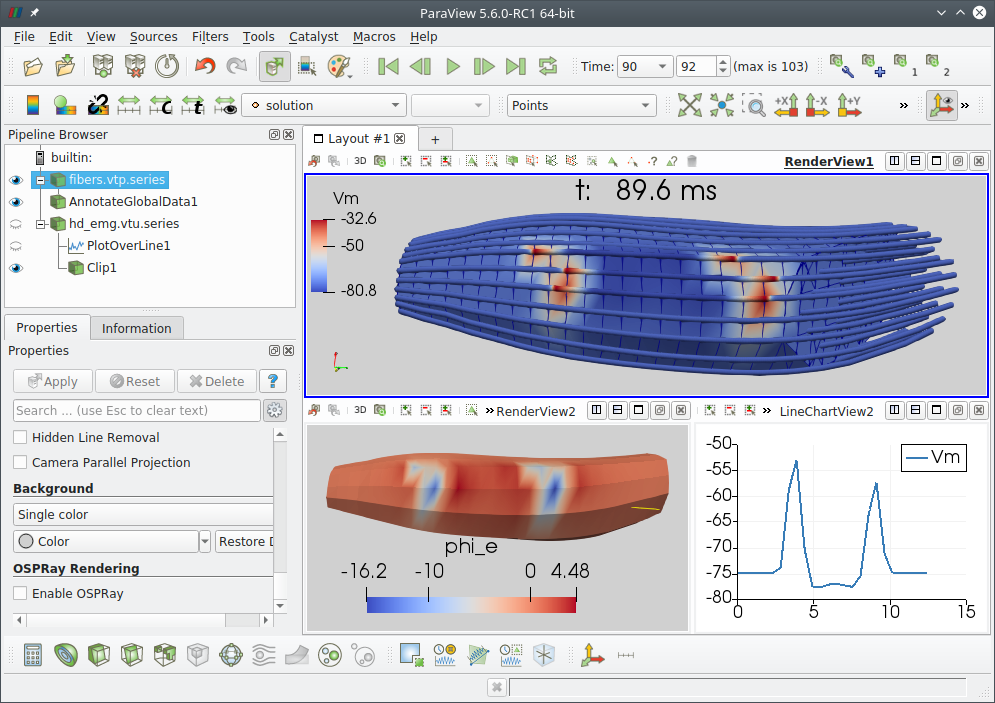
\includegraphics[width=\textwidth]{images/implementation/paraview.png}%
  \caption{Visualization of simulation results with ParaView: ParaView window with a visualization of muscle fibers and a 3D muscle mesh.}%
  \label{fig:paraview_output}%
\end{figure}%

The visualization in the center top view displays the membrane voltage $V_m$ at the fibers and in the 3D mesh, colored by the scheme shown at the left in the view. The 3D mesh is sliced on the right-hand side of the muscle to make the fiber dataset better visible.

The view on the bottom left depicts the extra-cellular potential $\phi_e$ on the 3D mesh. The view on the bottom right shows a plot of the value of $\phi_e$ along a horizontal line on the surface of the muscle.

It can be seen that three fibers near the surface are activated, and that the action potentials effect the EMG value given by $\phi_e$ on the surface.

For larger datasets, a head-less render server of ParaView also can be run in parallel on a remote server and the graphical user interface shown in \cref{fig:paraview_output} can be used as the client to interactively control the visualization.

ParaView also supports ray tracing using the OSPRay ray tracing engine. With ray tracing, more advanced lighting and the computation of shadows are possible.

\subsection{ExFiles and Visualization with CMGUI}

Another option in OpenDiHu is to output files in the \say{ExFile} format. This format originates from the software environment of OpenCMISS. Output of results in simulations with OpenCMISS Iron relies on this type of files. The visualization toolbox of OpenCMISS Zinc is able to create various visualizations of the data given in this format. The program \emph{CMGUI} provides a graphical user interface to visualize the data.

The output consists of corresponding \code{.exelem} and \code{.exnode} files containing information at element and node level, respectively. The mesh is assumed to be unstructured and, thus, the information which nodes correspond to a particular element has to be explicitly stored. It is stored in the \code{.exelem} file. The payload data are contained in the \code{.exnode} file. The file format supports parallel output to separate files. However, only serial output is supported in OpenDiHu.
ExFiles are ASCII-based and, thus, only usable up to a certain problem size.

An advantage of the \say{ExFile} format is that also higher order elements can be represented. The visualization tools are capable of representing the geometric data accordingly, e.g., it is possible to visualize the correct shape of cubic Hermite 3D hexahedral elements. In contrast, ParaView only visualizes linear elements and linearly interpolates the data between the nodes of an element.

The program CMGUI can be used to visualize the output files of OpenDiHu in ExFile format.
In the graphical user interface, the \code{.exelem} and \code{.exnode} files can be loaded. Representations of loaded points, lines and elements can be added to the visualization in the scene editor. Various options such as coordinate frames and parameters for shading and tessellation can be set. The visualizations can be colored using predefined appearances or according to the loaded solution values.

For larger datasets, these manual adjustments are tedious. For example, for a dataset with 49 fibers, the user would have to load 49 \code{.exelem} and 49 \code{.exnode} files one by one. Instead, the Perl scripting interface of CMGUI can be used. Every command in the GUI corresponds to a Perl command and CMGUI can load and execute those commands from a given Perl script.

OpenDiHu automatically creates such Perl scripts. The generated script for a mesh loads all generated output files into CMGUI, adds a  corresponding visualization depending on the mesh dimensionality and opens the required CMGUI windows such that the data are immediately visible. This is an improvement to OpenCMISS Iron, where all steps have to be done manually. By using the generated Perl script, less expert knowledge on the usage of CMGUI is required, and it is also possible to visualize datasets with a large number of fibers.

\Cref{fig:cmgui_output1} shows two windows of CMGUI. In \cref{fig:current_configuration_1}, the main graphics window can be seen with a visualization of 49 muscle fibers. The membrane potential is visualized by varying colors, and action potentials can be seen on three of the shown fibers. Similar to ParaView, the transient data can be animated by using the controls at the bottom.
\Cref{fig:cmgui_spectrum} shows the spectrum editor, where the color scheme can be adjusted to the range of the loaded data.

The other Perl script besides the one used in \cref{fig:cmgui_output1} to visualize the muscle fibers addresses the 3D mesh of the muscle.
\Cref{fig:cmgui_output2} shows the graphics windows with the resulting visualizations of this dataset. In \cref{fig:cmgui_emg}, the extracellular potential $\phi_e$ is visualized on the muscle surface. The visualization contains the colored 3D representation for the mesh and a 1D representation of the mesh consisting of white tubes.

\Cref{fig:cmgui_phie} demonstrates the feature of visualizing nodal data using glyphs. The $V_m$ values at every node are represented by colored circles with a radius that corresponds to the value. With this representation, it is possible to also show the data inside the muscle volume.

\begin{figure}%
  \centering%
  \begin{subfigure}[t]{0.62\textwidth}%
    \centering%
    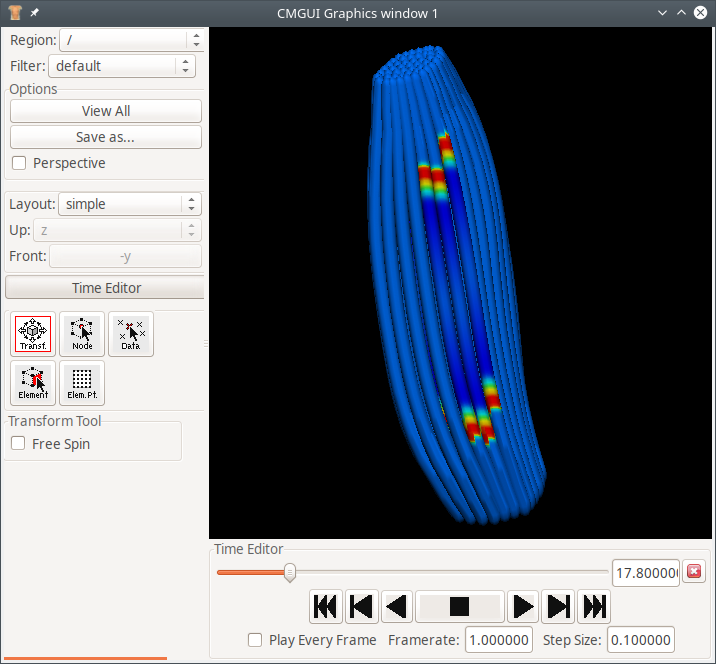
\includegraphics[width=\textwidth]{images/implementation/cmgui_graphics1.png}
    \caption{The main graphics window that displays the visualization and allows to control the current view and the current timestep.}%
    \label{fig:current_configuration_1}%
  \end{subfigure}
  \begin{subfigure}[t]{0.363\textwidth}%
    \centering%
    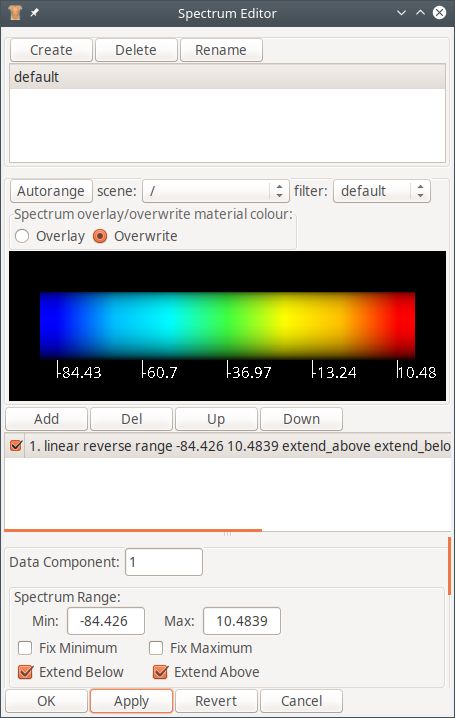
\includegraphics[width=\textwidth]{images/implementation/cmgui_spectrum.png}
    \caption{The spectrum editor that can be used to adjust the coloring according to the loaded solution values.}%
    \label{fig:cmgui_spectrum}%
  \end{subfigure}
  \caption{Visualization of the results of an electrophysiology simulation with CMGUI involving 49 muscle fibers.}%
  \label{fig:cmgui_output1}%
\end{figure}%

\begin{figure}%
  \centering%
  \begin{subfigure}[t]{0.48\textwidth}%
    \centering%
    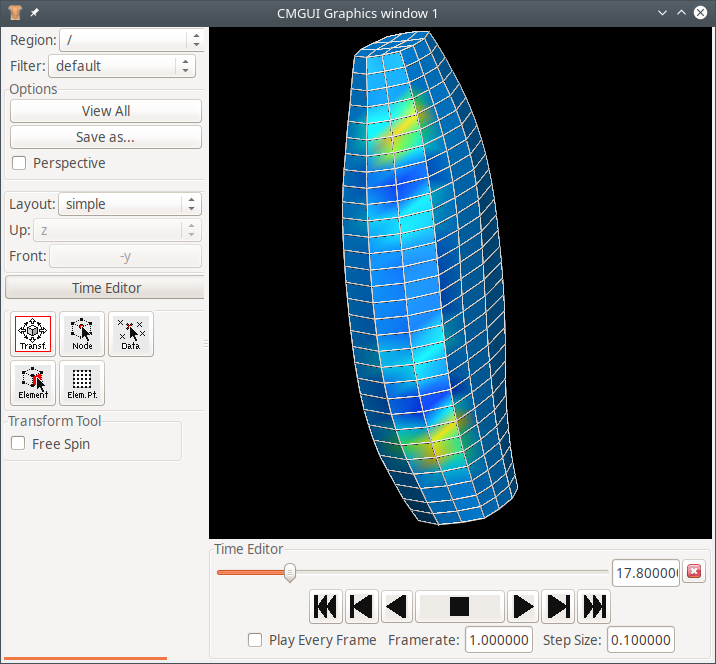
\includegraphics[width=\textwidth]{images/implementation/cmgui_emg.png}%
    \caption{Graphics window with the visualization of a 3D mesh.}%
    \label{fig:cmgui_emg}%
  \end{subfigure}
  \begin{subfigure}[t]{0.48\textwidth}%
    \centering%
    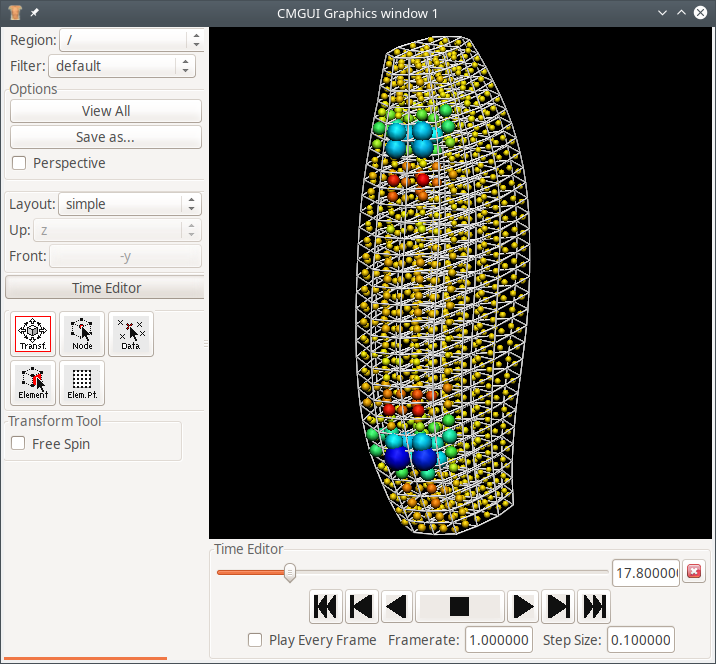
\includegraphics[width=\textwidth]{images/implementation/cmgui_phie.png}
    \caption{Visualization of the same data as in (a), but using sphere glyphs at every node.}%
    \label{fig:cmgui_phie}%
  \end{subfigure}
  \caption{Visualization of data on a 3D mesh with CMGUI.}%
  \label{fig:cmgui_output2}%
\end{figure}%

\subsection{Python Output Files}
Another option in OpenDiHu is to output data in a Python-friendly format, which can easily be parsed from within a python script.
The data can then be used, e.g., for error analysis or to convert them to other custom formats.

If the format \code{PythonFile} is specified in the output writer, the data get written to output files. If the format \code{PythonCallback} is specified, the same data are passed to a callback function and can directly be used in the Python settings script during the running simulation. 

For output, the data are organized in a Python dictionary. The output files either contain the plain Python code of this dictionary or a binary representation obtained by the \emph{pickle} package of Python. In parallel execution, every process writes its own file containing the data of the corresponding subdomain. OpenDiHu provides a Python module to parse these output files. The data representation, whether the data are stored in binary or in human-readable format and whether it is composed of multiple files resulting from parallel execution is abstracted and transparent in the call to this module.

The utility program \code{plot} can be used to quickly visualize the simulation results in such Python output files. It creates plots and animations of 1D and 2D structured meshes and chooses different layouts for the type of data, e.g, a plot over time for single-cell CellML models or an animation with multiple plots for subcellular models with multiple ion channels. This script is useful mainly for 1D and 2D toy problems, such as the Laplace, Poisson and Diffusion problems.

\Cref{fig:python_output} shows the output of the \code{plot} script for one muscle fiber. The top plot visualizes the geometry in 3D space, colored by the membrane potential $V_m$. The plot below shows the spatial progression of the $V_m$ value along the $x$-axis. However, for the visualization of 3D data, other options such as ParaView or CMGUI are better suited and should be used instead.

\begin{figure}%
  \centering%
  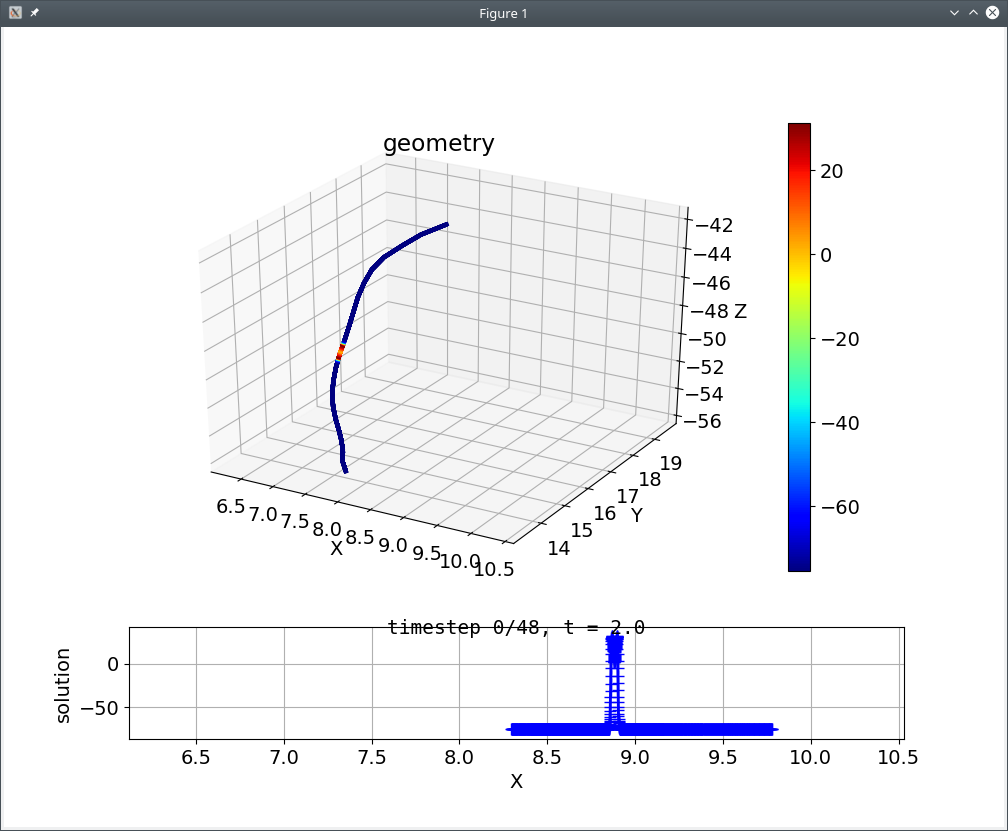
\includegraphics[width=\textwidth]{images/implementation/python_output.png}%
  \caption{Visualization of Python based simulation results using the \code{plot} utility.}%
  \label{fig:python_output}%
\end{figure}%

\subsection{ADIOS output files and MegaMol}
Another output format is the binary-pack file format defined by the Adaptable Input Output System library (ADIOS2). This type of output is selected by the OpenDiHu output writers for the \code{`MegaMol`} format. ADIOS2 provides a framework for high-performance computing data management \cite{adios2}. ADIOS2 manages self-describing data that allows rapid metadata extraction also from large data sets.

Output files in this format can be loaded into the visualization software MegaMol by experts. MegaMol has been successfully used together with OpenDiHu to implement in-situ visualization, where OpenDiHu shares the computed simulation data with MegaMol using the ADIOS2 format and triggers updates of the visualization by sending asynchronous messages to MegaMol during the runtime of the simulation. As both OpenDiHu and MegaMol can run in parallel, the partitioned data needs to be merged from all processes only at the stage of rendering the visualization image. For highly parallel runs on supercomputers, the local data that are generated by the OpenDiHu processes on the same compute node can be shared in memory with one instance of MegaMol per compute node. Then, all MegaMol instances collectively render the resulting visualization. This approach bypasses the costly file output operation on the highly distributed file system of a supercomputer.

\begin{figure}
\centering
\begin{framed}
%\begin{Verbatim}[fontsize=\small]
\begin{lstlisting}[basicstyle=\footnotesize\ttfamily,commentstyle=\color{gray},numbers=left,language=python]
    string   config                         (...)
    string   meta                           $\text{"}$current time: 2021/3/30 19:48:05,$\textcolor{gray}{\hookleftarrow}$
                                             hostname: lapsgs05, n ranks: 4$\text{"}$
    string   version                        $\text{"}$opendihu 1.2, built $\textcolor{gray}{\hookleftarrow}$
                                             Mar 27 2021, C++ 201402, GCC 7.5.0$\text{"}$
    double   localBoundingBox               10*{4, 6} = -56.3 / 19.7732   $\label{alg:7.6}$
    double   globalBoundingBox              10*{6} = -56.3 / 19.7732     $\label{alg:7.7}$
    double   global_radius                  10*scalar = 0.1 / 0.1
    int32_t  nPointsPerCoordinateDirection  10*{3} = 4 / 31
    int32_t  nodeOffsetOnOwnComputeNode     10*{4} = 0 / 368
    int32_t  node_count                     10*scalar = 496 / 496
    int32_t  rankNo                         10*{496} = 0 / 3                 $\label{alg:7.12}$
    double   emg                            10*{496} = -12.0536 / 4.89757    $\label{alg:7.13}$
    double   transmembraneFlow              10*{496} = -125.014 / 226.428    $\label{alg:7.14}$
    double   vm                             10*{496} = -81.3198 / -27.4762   $\label{alg:7.15}$
    double   xyz                            10*{1488} = -56.3 / 19.7732      $\label{alg:7.16}$
\end{lstlisting}
%\end{Verbatim}
\end{framed}
\caption{Contents of the output file created by ADIOS2.}%
\label{fig:adios_output}%
\end{figure}             

The generated output files can be inspected using the \code{bpls} utility. \Cref{fig:adios_output} shows a description of the 3D dataset extracted from the binary-pack format that was written by a simulation with four processes.
Each line corresponds to one variable in the file. The first column specifies the variable type and the second column is the name of the variable. The third column contains structural information with minimum and maximum values for numeric types. 

The first three shown variables are of type \code{string} and contain metadata for the simulation run. The \code{config} variable contains the Python settings code of the scenario and, thus, accurately describes the settings of the simulation run. 
The values of the \code{meta} and \code{version} variables are fully listed in \cref{fig:adios_output} and contain meta information about the simulation program and the particular run. 

For the numeric values, the third column specifies the dimension of the stored data. The file contains the simulation output for 10 different timesteps, which can be seen in the third column. For example, the \code{localBoundingBox} variable in line \ref{alg:7.6} stores 10 instances of a matrix with dimension $4\times 6$. The four rows of this matrix correspond to the four processes and the columns store the six values of the geometric bounding box of the subdomain on the respective process. This information is required by MegaMol to constrain the volume that has to be rendered on each process. Further structural information is contained in the variables in lines \ref{alg:7.7} to \ref{alg:7.12}. 
The remaining variables contain the payload data.  The variables \code{emg}, \code{transmembraneFlow} and \code{vm} correspond to $\phi_e$, the right-hand side of the first bidomain equation in \cref{eq:static_bidomain_rhs}, and $V_m$, respectively. The variable  \code{xyz} holds the geometry information for all nodes.


\begin{reproduce_no_break}
  The visualizations in this section are based on outputs of the following simulation:
  \begin{lstlisting}[columns=fullflexible,breaklines=true,postbreak=\mbox{\textcolor{gray}{$\hookrightarrow$}\space}]
    cd $\$$OPENDIHU_HOME/examples/electrophysiology/fibers/fibers_emg/build_release
    ./fast_fibers_emg ../settings_fibers_emg.py output_demo.py
  \end{lstlisting}
  
  Output files for ADIOS2, CMGUI, ParaView and Python will be generated in corresponding subdirectories under \code{out/}.
  The following commands invoke the respective visualization tool in the corresponding output directory:
  \begin{lstlisting}[columns=fullflexible,breaklines=true,postbreak=\mbox{\textcolor{gray}{$\hookrightarrow$}\space}]
    paraview fibers.vtp.series              # ParaView
    cmgui fibers.com                        # CMGUI
    cmgui hd_emg.com                        # CMGUI
    plot fibers_0000001_MeshFiber_*.py      # Python
    bpls hd_emg.bp -la                      # ADIOS2
  \end{lstlisting}
  In the graphical user interfaces of CMGUI and ParaView, more settings have to be adjusted to obtain the results shown in \cref{fig:paraview_output,fig:cmgui_output1,fig:cmgui_output2}.
  
  The listing shown in \cref{fig:adios_output} was obtained by a simulation with 4 processes. 
  Because the ExFile output writer does not work for parallel execution, the corresponding option has to be disabled in the \code{output_demo.py} variables file prior to execution:
  \begin{lstlisting}[columns=fullflexible,breaklines=true,postbreak=\mbox{\textcolor{gray}{$\hookrightarrow$}\space}]
    mpirun -n 4 ./fast_fibers_emg ../settings_fibers_emg.py output_demo.py
  \end{lstlisting}
  Afterwards, the shown listing can be obtained by \code{bpls -la hd_emg.bp}.
\end{reproduce_no_break}

